\documentclass[tikz,border=10pt]{standalone}
\usepackage{amsmath}
\usepackage{tikz}
\usetikzlibrary{shapes.geometric, arrows.meta, positioning}

\tikzstyle{block} = [rectangle, draw=blue!70, fill=blue!10, thick, minimum height=2em, minimum width=3.5cm, align=center]
\tikzstyle{central} = [rectangle, draw=black, thick, fill=gray!20, minimum width=4.5cm, align=center]
\tikzstyle{arrow} = [thick,->,>=stealth]

\begin{document}

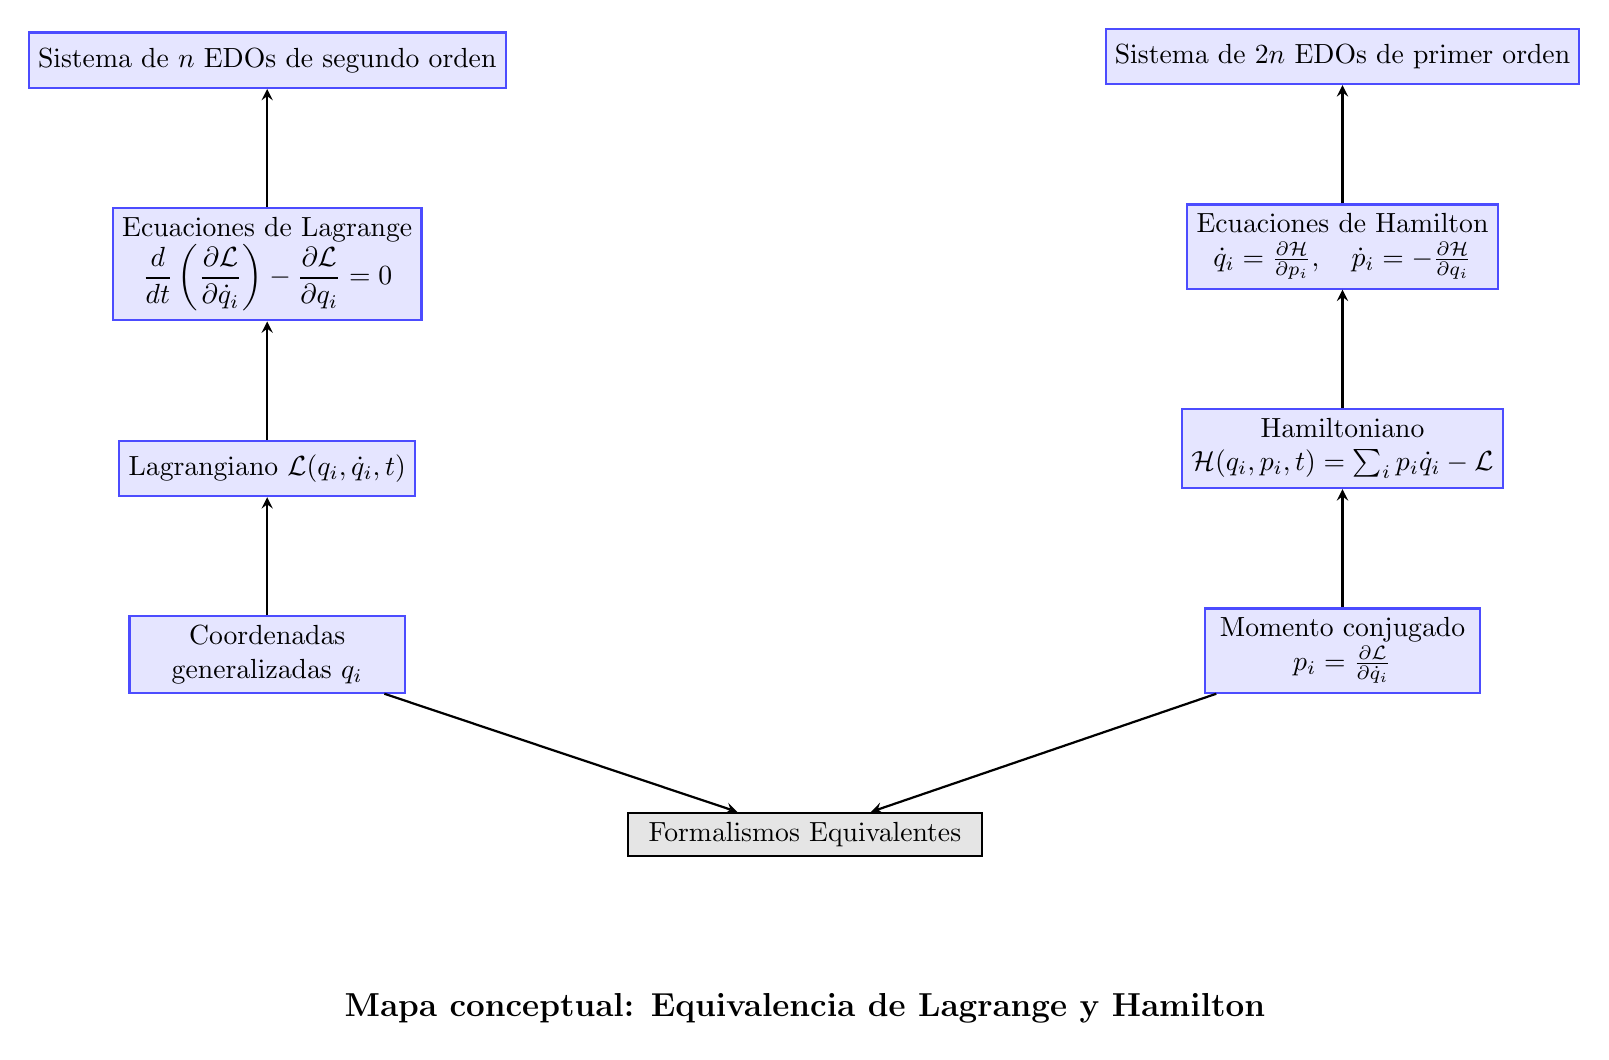
\begin{tikzpicture}[node distance=1.5cm and 2.8cm]

% Central box
\node (eq) [central] {Formalismos Equivalentes};

% Lagrangian branch
\node (lag1) [block, above left=of eq] {Coordenadas \\ generalizadas \( q_i \)};
\node (lag2) [block, above=of lag1] {Lagrangiano \( \mathcal{L}(q_i, \dot{q}_i, t) \)};
\node (lag3) [block, above=of lag2] {Ecuaciones de Lagrange \\
\(\displaystyle \frac{d}{dt} \left( \frac{\partial \mathcal{L}}{\partial \dot{q}_i} \right) - \frac{\partial \mathcal{L}}{\partial q_i} = 0\)};
\node (lag4) [block, above=of lag3] {Sistema de \( n \) EDOs de segundo orden};

% Hamiltonian branch
\node (ham1) [block, above right=of eq] {Momento conjugado \\
\( p_i = \frac{\partial \mathcal{L}}{\partial \dot{q}_i} \)};
\node (ham2) [block, above=of ham1] {Hamiltoniano \\
\( \mathcal{H}(q_i, p_i, t) = \sum_i p_i \dot{q}_i - \mathcal{L} \)};
\node (ham3) [block, above=of ham2] {Ecuaciones de Hamilton \\
\(\dot{q}_i = \frac{\partial \mathcal{H}}{\partial p_i}, \quad \dot{p}_i = -\frac{\partial \mathcal{H}}{\partial q_i} \)};
\node (ham4) [block, above=of ham3] {Sistema de \( 2n \) EDOs de primer orden};

% Arrows Lagrangian
\draw [arrow] (lag1) -- (lag2);
\draw [arrow] (lag2) -- (lag3);
\draw [arrow] (lag3) -- (lag4);
\draw [arrow] (lag1) -- (eq);

% Arrows Hamiltonian
\draw [arrow] (ham1) -- (ham2);
\draw [arrow] (ham2) -- (ham3);
\draw [arrow] (ham3) -- (ham4);
\draw [arrow] (ham1) -- (eq);

% Title
\node at (0,-2.2) {\large \textbf{Mapa conceptual: Equivalencia de Lagrange y Hamilton}};

\end{tikzpicture}

\end{document}


\documentclass{article}
\usepackage[utf8]{inputenc}
\usepackage{amsmath}
\usepackage{array}
\usepackage{geometry}
\geometry{margin=1in}

\begin{document}

\renewcommand{\arraystretch}{1.6}
\begin{center}
\textbf{\Large Equivalencia de los Formalismos de Lagrange y Hamilton}
\end{center}

\begin{tabular}{|>{\raggedright\arraybackslash}p{2cm}|>{\raggedright\arraybackslash}p{6.5cm}|>{\raggedright\arraybackslash}p{6.5cm}|}
\hline
\textbf{Paso} & \textbf{Formalismo Lagrangiano} & \textbf{Formalismo Hamiltoniano} \\
\hline
1 & Elegir coordenadas generalizadas \( q_i \) & Usar las mismas \( q_i \) y definir los momentos conjugados \( p_i = \frac{\partial \mathcal{L}}{\partial \dot{q}_i} \) \\
\hline
2 & Escribir el lagrangiano \( \mathcal{L}(q_i, \dot{q}_i, t) = T - V \) & Calcular el hamiltoniano \( \mathcal{H}(q_i, p_i, t) = \sum_i \dot{q}_i p_i - L \) \\
\hline
3 & Obtener las ecuaciones de Euler-Lagrange: 
\( \frac{d}{dt} \left( \frac{\partial \mathcal{L}}{\partial \dot{q}_i} \right) - \frac{\partial \mathcal{L}}{\partial q_i} = 0 \) & Usar las ecuaciones de Hamilton:
\( \dot{q}_i = \frac{\partial \mathcal{H}}{\partial p_i}, \quad \dot{p}_i = -\frac{\partial \mathcal{H}}{\partial q_i} \) \\
\hline
4 & Resolver ecuaciones diferenciales de segundo orden para \( q_i(t) \) & Resolver ecuaciones acopladas de primer orden para \( q_i(t) \), \( p_i(t) \) \\
\hline
5 & Las cantidades conservadas surgen de coordenadas c�clicas \( q_i \) & Las cantidades conservadas se obtienen a partir de simetr�as de \( H \) \\
\hline
6 & Imagen geom�trica: espacio de configuraci�n \( (q_i) \) & Imagen geom�trica: espacio de fases \( (q_i, p_i) \) \\
\hline
7 & Simetr�as mediante el teorema de Noether & Simetr�as mediante transformaciones can�nicas \\
\hline
\end{tabular}

\end{document}

